\documentclass[12pt,letterpaper]{exam}
\usepackage[lmargin=1in,rmargin=1in,tmargin=1in,bmargin=1in]{geometry}
\usepackage{../style/exams}

% -------------------
% Course & Exam Information
% -------------------
\newcommand{\course}{MAT 104: Exam 1}
\newcommand{\term}{Spring -- 2023}
\newcommand{\examdate}{03/03/2023}
\newcommand{\timelimit}{85 Minutes}

\setbool{hideans}{true} % Student: True; Instructor: False

% -------------------
% Content
% -------------------
\begin{document}

\examtitle
\instructions{Write your name on the appropriate line on the exam cover sheet. This exam contains \numpages\ pages (including this cover page) and \numquestions\ questions. Check that you have every page of the exam. Answer the questions in the spaces provided on the question sheets. Be sure to answer every part of each question and show all your work.} 
\scores
%\bottomline
\newpage

% ---------
% Questions
% ---------
\begin{questions}

% Question 1
\newpage
\question[10] Suppose that $f(x)$ is a function with domain $[-10, 10)$ and $g(x)$ is a function with domain $(-5, 15]$. Several outputs for the functions $f(x)$ and $g(x)$ are given below. \par
	\begin{table}[!ht]
	\centering
	\begin{tabular}{|c||c|c|c|c|c|} \hline
	$x$ & $0$ & $1$ & $2$ & $3$ & $5$ \\ \hline \hline
	$f(x)$ & $3$ & $0$ & $2$ & $4$ & $4$ \\ \hline
	$g(x)$ & $3$ & $5$ & $1$ & $2$ & $0$ \\ \hline
	\end{tabular}
	\end{table} \par

\begin{enumerate}[(a)]
\item What is the domain of $f - g$?
\item Given the information above, what is the largest possible domain for $\frac{f}{g}$?
\item Find $(f + g)(2)$.
\item Find $(fg)(0)$.
\item Find $(g \circ f)(0)$.
\end{enumerate}



% Question 2
\newpage
\question[10] Let $f(x)$ be an exponential function with $f(-2)= 12$ and $f(3)= \frac{3}{8}$. Showing all your work, find $f(x)$. 



% Question 3
\newpage
\question[10] Showing all your work, find the inverse of the function $f(x)= \log_3(x^2) - 4$.



% Question 4
\newpage
\question[10] A function $f(x)$ is plotted below. As accurately as possible, sketch the function $4 - f(x + 3)$ on the graph below. 
	\[
	\fbox{
	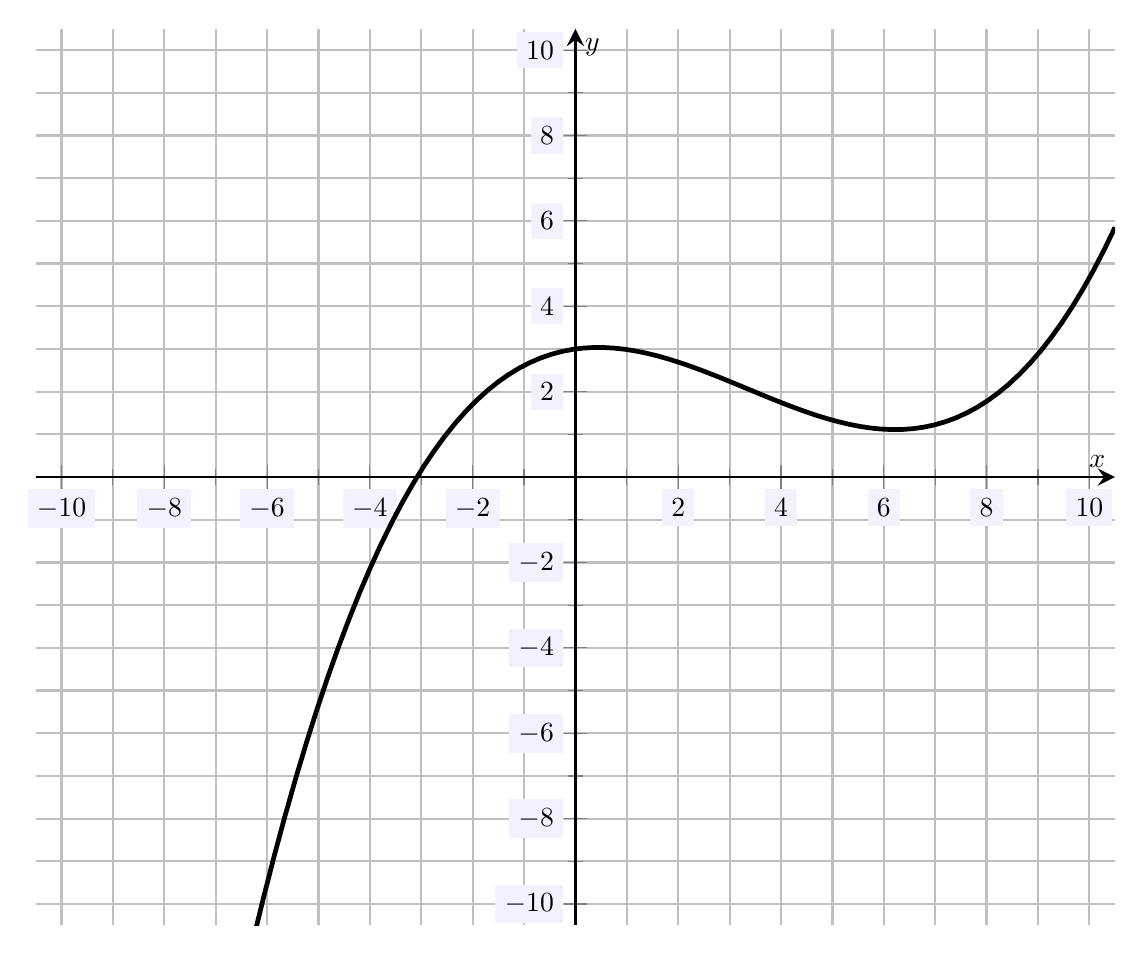
\begin{tikzpicture}[scale=2,every node/.style={scale=0.5}]
	\begin{axis}[
	grid=both,
	axis lines=middle,
	ticklabel style={fill=blue!5!white},
	xmin= -10.5, xmax=10.5,
	ymin= -10.5, ymax=10.5,
	xtick={-10,-8,...,10},
	ytick={-10,-8,...,10},
	minor x tick num = 1,
	minor y tick num = 1,
	xlabel=\(x\),ylabel=\(y\),
	]
	\addplot[domain=-10:10.5,samples=100,line width=0.03cm] (x,1/50*x^3 - 1/5*x^2 + 1/6*x + 3);
	\end{axis}
	\end{tikzpicture}
	}
	\] 



% Question 5
\newpage
\question[10] Let $f(x)= 3 - 2x$ and $g(x)= x^2 + x - 1$. Showing all your work and simplifying as much as possible, find the following:
	\begin{enumerate}[(a)]
	\item $f \big( g(0) \big)$
	\item $(2f - g)(0)$
	\item $(g - f)(x)$
	\item $(f \circ g)(x)$
	\item $(g \circ f)(x)$
	\end{enumerate}



% Question 6
\newpage
\question[10] Showing all your work, find the inverse of the function $f(x)= 3e^{1 - 2x}$.



% Question 7
\newpage
\question[10] Let $f(x)$ be the function $f(x)= \dfrac{2^{3x + 1}}{5^{1 - x}}$.
	\begin{enumerate}[(a)]
	\item Write $f(x)$ in the form $ab^x$ for some $a$, $b$. 
	\item Is $f(x)$ increasing or decreasing?
	\item Is $f(x)$ concave up or concave down?
	\end{enumerate}



% Question 8
\newpage
\question[10] Showing all your work, find the exact solution to the following:
	\[
	\log_2 \left( 50 - e^{x + 1} \right) + 5= 10
	\]



% Question 9
\newpage
\question[10] Showing all your work, write the following as a sum of terms involving only $\log_2(x)$, $\log_2(y)$, and possibly a constant:
	\[
	\log_2 \left( \dfrac{16 \sqrt[3]{x}}{y^{-5}} \right)
	\]



% Question 10
\newpage
\question[10] Let $f(x)= 2 - e^x$ and $g(x)= 6 \log_5( 2 - x)$.
	\begin{enumerate}[(a)]
	\item What is the domain of $f(x)$?
	\item What is the range of $f(x)$?
	\item What is the domain of $g(x)$?
	\item What is the range of $g(x)$?
	\end{enumerate}



% Question 11
\newpage
\question[10] Showing all your work, find the exact solution to the following:
	\[
	3^{2x}= 5 \cdot 2^x
	\]



% Question 12
\newpage
\question[10] A relation $f(x)$ is plotted below.
	\[
	\fbox{
	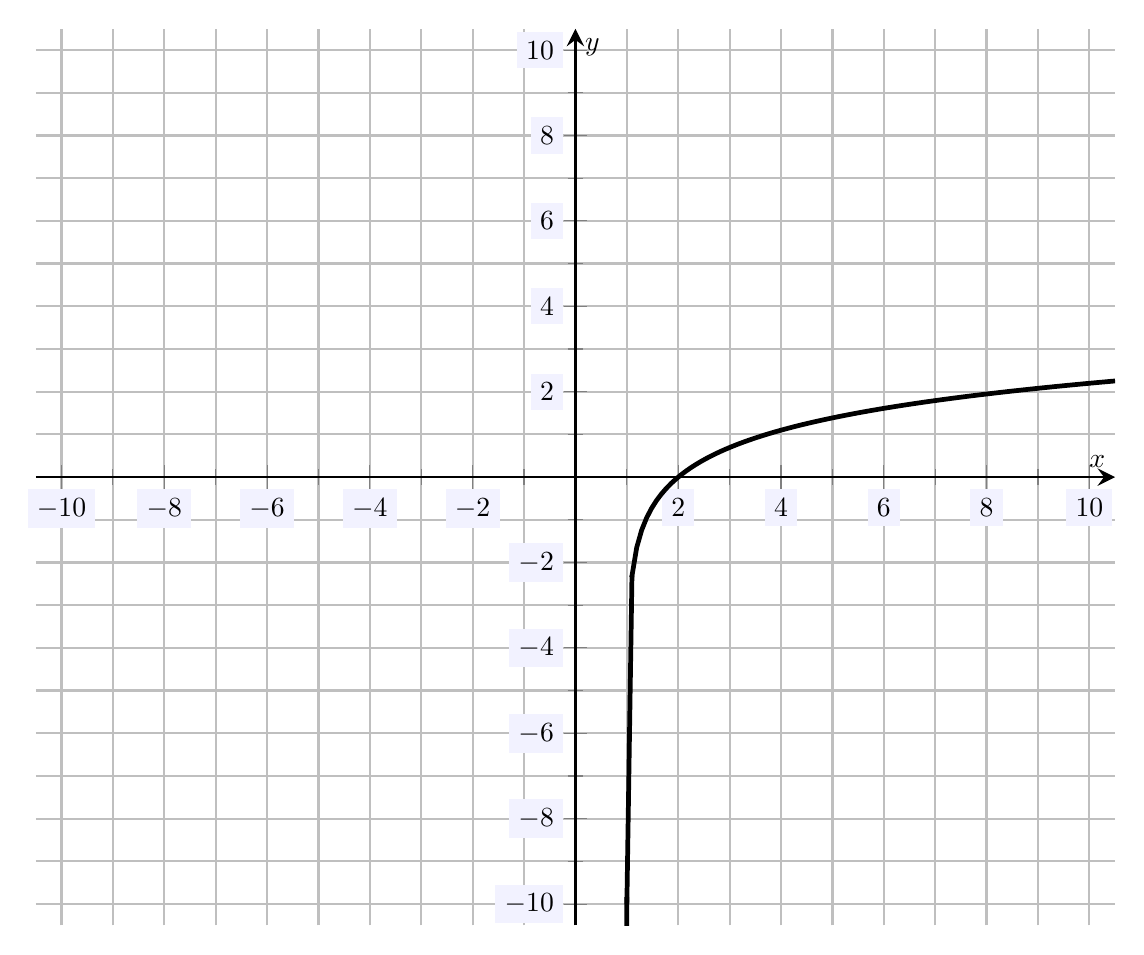
\begin{tikzpicture}[scale=2,every node/.style={scale=0.5}]
	\begin{axis}[
	grid=both,
	axis lines=middle,
	ticklabel style={fill=blue!5!white},
	xmin= -10.5, xmax=10.5,
	ymin= -10.5, ymax=10.5,
	xtick={-10,-8,...,10},
	ytick={-10,-8,...,10},
	minor x tick num = 1,
	minor y tick num = 1,
	xlabel=\(x\),ylabel=\(y\),
	]
	\addplot[domain=1:10.5,samples=100,line width=0.03cm] {ln(x - 1)};
	\addplot[domain=1:1.00005,samples=100,line width=0.03cm] {ln(x - 1)};
	\draw[line width=0.03cm] (1.0006,-10) -- (1.1,-2.3);
	\end{axis}
	\end{tikzpicture}
	}
	\] 
\begin{enumerate}[(a)]
\item Using the plot above, explain why $f(x)$ is a function.
\item Using the plot above, explain why $f^{-1}(x)$ exists.
\item Sketch the function $f^{-1}(x)$ on the plot above. 
\end{enumerate}



% Question 13
\newpage
\question[10] Showing all your work, write each of the following as a single logarithm involving no negative powers:
	\begin{enumerate}[(a)]
	\item $\ln(x) + 3 \ln(y)$
	\item $\log_5(x) - \log_5(y^{-2})$
	\item $4\log_3(x) - \frac{1}{2} \log_3(y) + 2$
	\end{enumerate}


% Question 14
\newpage
\question[10] Showing all your work, compute the following ``by hand'': 
	\begin{enumerate}[(a)]
	\item $\ln(e^{3/2})$
	\item $\log_3(\sqrt{5})$
	\item $\log_4 \left( \frac{1}{64} \right)$
	\item $\log_9(3)$
	\item $\log_8(128)$
	\end{enumerate}



% Question 15
\newpage
\question[10] If one invests $P$ dollars at an annual interest rate $r$ (written as a decimal), compounded monthly, then the amount of money in the account after $t$ years, $M(t)$, is given by\dots
	\[
	M(t)= P \left(1 + \dfrac{r}{12} \right)^{12t}
	\]
Suppose that you invest \$8,000 at an annual interest rate of 6.2\%, compounded monthly. 

\begin{enumerate}[(a)]
\item Find the value of the investment after 5~years.
\item Find how long until the investment is worth \$20,000. 
\end{enumerate}


\end{questions}
\end{document}